
%% bare_conf.tex
%% V1.3
%% 2007/01/11
%% by Michael Shell
%% See:
%% http://www.michaelshell.org/
%% for current contact information.
%%
%% This is a skeleton file demonstrating the use of IEEEtran.cls
%% (requires IEEEtran.cls version 1.7 or later) with an IEEE conference paper.
%%
%% Support sites:
%% http://www.michaelshell.org/tex/ieeetran/
%% http://www.ctan.org/tex-archive/macros/latex/contrib/IEEEtran/
%% and
%% http://www.ieee.org/

%%*************************************************************************
%% Legal Notice:
%% This code is offered as-is without any warranty either expressed or
%% implied; without even the implied warranty of MERCHANTABILITY or
%% FITNESS FOR A PARTICULAR PURPOSE! 
%% User assumes all risk.
%% In no event shall IEEE or any contributor to this code be liable for
%% any damages or losses, including, but not limited to, incidental,
%% consequential, or any other damages, resulting from the use or misuse
%% of any information contained here.
%%
%% All comments are the opinions of their respective authors and are not
%% necessarily endorsed by the IEEE.
%%
%% This work is distributed under the LaTeX Project Public License (LPPL)
%% ( http://www.latex-project.org/ ) version 1.3, and may be freely used,
%% distributed and modified. A copy of the LPPL, version 1.3, is included
%% in the base LaTeX documentation of all distributions of LaTeX released
%% 2003/12/01 or later.
%% Retain all contribution notices and credits.
%% ** Modified files should be clearly indicated as such, including  **
%% ** renaming them and changing author support contact information. **
%%
%% File list of work: IEEEtran.cls, IEEEtran_HOWTO.pdf, bare_adv.tex,
%%                    bare_conf.tex, bare_jrnl.tex, bare_jrnl_compsoc.tex
%%*************************************************************************

% *** Authors should verify (and, if needed, correct) their LaTeX system  ***
% *** with the testflow diagnostic prior to trusting their LaTeX platform ***
% *** with production work. IEEE's font choices can trigger bugs that do  ***
% *** not appear when using other class files.                            ***
% The testflow support page is at:
% http://www.michaelshell.org/tex/testflow/



% Note that the a4paper option is mainly intended so that authors in
% countries using A4 can easily print to A4 and see how their papers will
% look in print - the typesetting of the document will not typically be
% affected with changes in paper size (but the bottom and side margins will).
% Use the testflow package mentioned above to verify correct handling of
% both paper sizes by the user's LaTeX system.
%
% Also note that the "draftcls" or "draftclsnofoot", not "draft", option
% should be used if it is desired that the figures are to be displayed in
% draft mode.
%
\documentclass[conference]{IEEEtran}
% Add the compsoc option for Computer Society conferences.
%
% If IEEEtran.cls has not been installed into the LaTeX system files,
% manually specify the path to it like:
% \documentclass[conference]{../sty/IEEEtran}





% Some very useful LaTeX packages include:
% (uncomment the ones you want to load)


% *** MISC UTILITY PACKAGES ***
%
%\usepackage{ifpdf}
% Heiko Oberdiek's ifpdf.sty is very useful if you need conditional
% compilation based on whether the output is pdf or dvi.
% usage:
% \ifpdf
%   % pdf code
% \else
%   % dvi code
% \fi
% The latest version of ifpdf.sty can be obtained from:
% http://www.ctan.org/tex-archive/macros/latex/contrib/oberdiek/
% Also, note that IEEEtran.cls V1.7 and later provides a builtin
% \ifCLASSINFOpdf conditional that works the same way.
% When switching from latex to pdflatex and vice-versa, the compiler may
% have to be run twice to clear warning/error messages.






% *** CITATION PACKAGES ***
%
%\usepackage{cite}
% cite.sty was written by Donald Arseneau
% V1.6 and later of IEEEtran pre-defines the format of the cite.sty package
% \cite{} output to follow that of IEEE. Loading the cite package will
% result in citation numbers being automatically sorted and properly
% "compressed/ranged". e.g., [1], [9], [2], [7], [5], [6] without using
% cite.sty will become [1], [2], [5]--[7], [9] using cite.sty. cite.sty's
% \cite will automatically add leading space, if needed. Use cite.sty's
% noadjust option (cite.sty V3.8 and later) if you want to turn this off.
% cite.sty is already installed on most LaTeX systems. Be sure and use
% version 4.0 (2003-05-27) and later if using hyperref.sty. cite.sty does
% not currently provide for hyperlinked citations.
% The latest version can be obtained at:
% http://www.ctan.org/tex-archive/macros/latex/contrib/cite/
% The documentation is contained in the cite.sty file itself.






% *** GRAPHICS RELATED PACKAGES ***
%
\ifCLASSINFOpdf
  % \usepackage[pdftex]{graphicx}
  % declare the path(s) where your graphic files are
  % \graphicspath{{../pdf/}{../jpeg/}}
  % and their extensions so you won't have to specify these with
  % every instance of \includegraphics
  % \DeclareGraphicsExtensions{.pdf,.jpeg,.png}
\else
  % or other class option (dvipsone, dvipdf, if not using dvips). graphicx
  % will default to the driver specified in the system graphics.cfg if no
  % driver is specified.
  \usepackage[dvips]{graphicx}
  % declare the path(s) where your graphic files are
  \graphicspath{{./figures/}}
  % and their extensions so you won't have to specify these with
  % every instance of \includegraphics
  \DeclareGraphicsExtensions{.eps}
\fi
% graphicx was written by David Carlisle and Sebastian Rahtz. It is
% required if you want graphics, photos, etc. graphicx.sty is already
% installed on most LaTeX systems. The latest version and documentation can
% be obtained at: 
% http://www.ctan.org/tex-archive/macros/latex/required/graphics/
% Another good source of documentation is "Using Imported Graphics in
% LaTeX2e" by Keith Reckdahl which can be found as epslatex.ps or
% epslatex.pdf at: http://www.ctan.org/tex-archive/info/
%
% latex, and pdflatex in dvi mode, support graphics in encapsulated
% postscript (.eps) format. pdflatex in pdf mode supports graphics
% in .pdf, .jpeg, .png and .mps (metapost) formats. Users should ensure
% that all non-photo figures use a vector format (.eps, .pdf, .mps) and
% not a bitmapped formats (.jpeg, .png). IEEE frowns on bitmapped formats
% which can result in "jaggedy"/blurry rendering of lines and letters as
% well as large increases in file sizes.
%
% You can find documentation about the pdfTeX application at:
% http://www.tug.org/applications/pdftex





% *** MATH PACKAGES ***
%
\usepackage[cmex10]{amsmath}
% A popular package from the American Mathematical Society that provides
% many useful and powerful commands for dealing with mathematics. If using
% it, be sure to load this package with the cmex10 option to ensure that
% only type 1 fonts will utilized at all point sizes. Without this option,
% it is possible that some math symbols, particularly those within
% footnotes, will be rendered in bitmap form which will result in a
% document that can not be IEEE Xplore compliant!
%
% Also, note that the amsmath package sets \interdisplaylinepenalty to 10000
% thus preventing page breaks from occurring within multiline equations. Use:
%\interdisplaylinepenalty=2500
% after loading amsmath to restore such page breaks as IEEEtran.cls normally
% does. amsmath.sty is already installed on most LaTeX systems. The latest
% version and documentation can be obtained at:
% http://www.ctan.org/tex-archive/macros/latex/required/amslatex/math/





% *** SPECIALIZED LIST PACKAGES ***
%
%\usepackage{algorithmic}
% algorithmic.sty was written by Peter Williams and Rogerio Brito.
% This package provides an algorithmic environment fo describing algorithms.
% You can use the algorithmic environment in-text or within a figure
% environment to provide for a floating algorithm. Do NOT use the algorithm
% floating environment provided by algorithm.sty (by the same authors) or
% algorithm2e.sty (by Christophe Fiorio) as IEEE does not use dedicated
% algorithm float types and packages that provide these will not provide
% correct IEEE style captions. The latest version and documentation of
% algorithmic.sty can be obtained at:
% http://www.ctan.org/tex-archive/macros/latex/contrib/algorithms/
% There is also a support site at:
% http://algorithms.berlios.de/index.html
% Also of interest may be the (relatively newer and more customizable)
% algorithmicx.sty package by Szasz Janos:
% http://www.ctan.org/tex-archive/macros/latex/contrib/algorithmicx/




% *** ALIGNMENT PACKAGES ***
%
%\usepackage{array}
% Frank Mittelbach's and David Carlisle's array.sty patches and improves
% the standard LaTeX2e array and tabular environments to provide better
% appearance and additional user controls. As the default LaTeX2e table
% generation code is lacking to the point of almost being broken with
% respect to the quality of the end results, all users are strongly
% advised to use an enhanced (at the very least that provided by array.sty)
% set of table tools. array.sty is already installed on most systems. The
% latest version and documentation can be obtained at:
% http://www.ctan.org/tex-archive/macros/latex/required/tools/


%\usepackage{mdwmath}
%\usepackage{mdwtab}
% Also highly recommended is Mark Wooding's extremely powerful MDW tools,
% especially mdwmath.sty and mdwtab.sty which are used to format equations
% and tables, respectively. The MDWtools set is already installed on most
% LaTeX systems. The lastest version and documentation is available at:
% http://www.ctan.org/tex-archive/macros/latex/contrib/mdwtools/


% IEEEtran contains the IEEEeqnarray family of commands that can be used to
% generate multiline equations as well as matrices, tables, etc., of high
% quality.


%\usepackage{eqparbox}
% Also of notable interest is Scott Pakin's eqparbox package for creating
% (automatically sized) equal width boxes - aka "natural width parboxes".
% Available at:
% http://www.ctan.org/tex-archive/macros/latex/contrib/eqparbox/





% *** SUBFIGURE PACKAGES ***
%\usepackage[tight,footnotesize]{subfigure}
% subfigure.sty was written by Steven Douglas Cochran. This package makes it
% easy to put subfigures in your figures. e.g., "Figure 1a and 1b". For IEEE
% work, it is a good idea to load it with the tight package option to reduce
% the amount of white space around the subfigures. subfigure.sty is already
% installed on most LaTeX systems. The latest version and documentation can
% be obtained at:
% http://www.ctan.org/tex-archive/obsolete/macros/latex/contrib/subfigure/
% subfigure.sty has been superceeded by subfig.sty.



%\usepackage[caption=false]{caption}
%\usepackage[font=footnotesize]{subfig}
% subfig.sty, also written by Steven Douglas Cochran, is the modern
% replacement for subfigure.sty. However, subfig.sty requires and
% automatically loads Axel Sommerfeldt's caption.sty which will override
% IEEEtran.cls handling of captions and this will result in nonIEEE style
% figure/table captions. To prevent this problem, be sure and preload
% caption.sty with its "caption=false" package option. This is will preserve
% IEEEtran.cls handing of captions. Version 1.3 (2005/06/28) and later 
% (recommended due to many improvements over 1.2) of subfig.sty supports
% the caption=false option directly:
%\usepackage[caption=false,font=footnotesize]{subfig}
%
% The latest version and documentation can be obtained at:
% http://www.ctan.org/tex-archive/macros/latex/contrib/subfig/
% The latest version and documentation of caption.sty can be obtained at:
% http://www.ctan.org/tex-archive/macros/latex/contrib/caption/




% *** FLOAT PACKAGES ***
%
%\usepackage{fixltx2e}
% fixltx2e, the successor to the earlier fix2col.sty, was written by
% Frank Mittelbach and David Carlisle. This package corrects a few problems
% in the LaTeX2e kernel, the most notable of which is that in current
% LaTeX2e releases, the ordering of single and double column floats is not
% guaranteed to be preserved. Thus, an unpatched LaTeX2e can allow a
% single column figure to be placed prior to an earlier double column
% figure. The latest version and documentation can be found at:
% http://www.ctan.org/tex-archive/macros/latex/base/



%\usepackage{stfloats}
% stfloats.sty was written by Sigitas Tolusis. This package gives LaTeX2e
% the ability to do double column floats at the bottom of the page as well
% as the top. (e.g., "\begin{figure*}[!b]" is not normally possible in
% LaTeX2e). It also provides a command:
%\fnbelowfloat
% to enable the placement of footnotes below bottom floats (the standard
% LaTeX2e kernel puts them above bottom floats). This is an invasive package
% which rewrites many portions of the LaTeX2e float routines. It may not work
% with other packages that modify the LaTeX2e float routines. The latest
% version and documentation can be obtained at:
% http://www.ctan.org/tex-archive/macros/latex/contrib/sttools/
% Documentation is contained in the stfloats.sty comments as well as in the
% presfull.pdf file. Do not use the stfloats baselinefloat ability as IEEE
% does not allow \baselineskip to stretch. Authors submitting work to the
% IEEE should note that IEEE rarely uses double column equations and
% that authors should try to avoid such use. Do not be tempted to use the
% cuted.sty or midfloat.sty packages (also by Sigitas Tolusis) as IEEE does
% not format its papers in such ways.





% *** PDF, URL AND HYPERLINK PACKAGES ***
%
\usepackage{url}
% url.sty was written by Donald Arseneau. It provides better support for
% handling and breaking URLs. url.sty is already installed on most LaTeX
% systems. The latest version can be obtained at:
% http://www.ctan.org/tex-archive/macros/latex/contrib/misc/
% Read the url.sty source comments for usage information. Basically,
% \url{my_url_here}.





% *** Do not adjust lengths that control margins, column widths, etc. ***
% *** Do not use packages that alter fonts (such as pslatex).         ***
% There should be no need to do such things with IEEEtran.cls V1.6 and later.
% (Unless specifically asked to do so by the journal or conference you plan
% to submit to, of course. )


% correct bad hyphenation here
\hyphenation{op-tical net-works semi-conduc-tor}


\begin{document}
%
% paper title
% can use linebreaks \\ within to get better formatting as desired
\title{A Revolutionary New Paradigm for the Reduction and Analysis of Astronomical Images}


% author names and affiliations
% use a multiple column layout for up to three different
% affiliations
\author{\IEEEauthorblockN{Scott Michael}
\IEEEauthorblockA{Indiana University\\
Bloomington, Indiana 47408\\
Email: scamicha@indiana.edu}
\and
\IEEEauthorblockN{Homer Simpson}
\IEEEauthorblockA{Twentieth Century Fox\\
Springfield, USA\\
Email: homer@thesimpsons.com}
\and
\IEEEauthorblockN{James Kirk\\ and Montgomery Scott}
\IEEEauthorblockA{Starfleet Academy\\
San Francisco, California 96678-2391\\
Telephone: (800) 555--1212\\
Fax: (888) 555--1212}}

% conference papers do not typically use \thanks and this command
% is locked out in conference mode. If really needed, such as for
% the acknowledgment of grants, issue a \IEEEoverridecommandlockouts
% after \documentclass

% for over three affiliations, or if they all won't fit within the width
% of the page, use this alternative format:
% 
%\author{\IEEEauthorblockN{Michael Shell\IEEEauthorrefmark{1},
%Homer Simpson\IEEEauthorrefmark{2},
%James Kirk\IEEEauthorrefmark{3}, 
%Montgomery Scott\IEEEauthorrefmark{3} and
%Eldon Tyrell\IEEEauthorrefmark{4}}
%\IEEEauthorblockA{\IEEEauthorrefmark{1}School of Electrical and Computer Engineering\\
%Georgia Institute of Technology,
%Atlanta, Georgia 30332--0250\\ Email: see http://www.michaelshell.org/contact.html}
%\IEEEauthorblockA{\IEEEauthorrefmark{2}Twentieth Century Fox, Springfield, USA\\
%Email: homer@thesimpsons.com}
%\IEEEauthorblockA{\IEEEauthorrefmark{3}Starfleet Academy, San Francisco, California 96678-2391\\
%Telephone: (800) 555--1212, Fax: (888) 555--1212}
%\IEEEauthorblockA{\IEEEauthorrefmark{4}Tyrell Inc., 123 Replicant Street, Los Angeles, California 90210--4321}}




% use for special paper notices
%\IEEEspecialpapernotice{(Invited Paper)}




% make the title area
\maketitle


\begin{abstract}
%\boldmath
The abstract goes here.
\end{abstract}
% IEEEtran.cls defaults to using nonbold math in the Abstract.
% This preserves the distinction between vectors and scalars. However,
% if the conference you are submitting to favors bold math in the abstract,
% then you can use LaTeX's standard command \boldmath at the very start
% of the abstract to achieve this. Many IEEE journals/conferences frown on
% math in the abstract anyway.

% no keywords




% For peer review papers, you can put extra information on the cover
% page as needed:
% \ifCLASSOPTIONpeerreview
% \begin{center} \bfseries EDICS Category: 3-BBND \end{center}
% \fi
%
% For peerreview papers, this IEEEtran command inserts a page break and
% creates the second title. It will be ignored for other modes.
\IEEEpeerreviewmaketitle



\section{Introduction}\label{sec:intro}
However, cutting-edge instruments that are just beginning to come online, as well as instruments planned for the not too distant future will produce data in volumes that a single investigator can not hope to store, analyze, and archive on their own. Currently, the Pan-STARRS gigapixel imager is producing more than 1 TB of data per day. The Solar Dynamics Observatory, a space based observatory, transmits 1.5 TB of raw data to the ground every day. Other instruments in their design or construction phases include the One Degree Imager, capable of producing 4 TB per day; the Large Synoptic Sky Survey, which will produce 30 TB of data per day; and the Joint Dark Energy Mission, a space based observatory capable of producing several terabytes of data per day. Clearly, these data volumes are much larger than the typical astronomer is accustomed to dealing with and most observational astronomers lack access to the resources that would be required to handle these amounts of data. 

To address this changing landscape of data output from leading scientific observatories, we propose a new paradigm for the storage, analysis and archiving of astronomical digital image data. By taking advantage of 

The rest of this paper is arranged as follows: \S\ref{sec:current} describes the current paradigm employed by astronomers for dealing with imaging data and outline some upcoming problems with this paradigm. We detail a new paradigm for the processing of astronomical images in \S\ref{sec:rev}. In \S\ref{sec:ODI} we describe how this new paradigm applies to the ODI instrument. Finally, in \S\ref{sec:future} we explore possible future directions and in \S\ref{sec:conclusions} we present our final conclusions.

\section{The Current Paradigm for the Reduction of Astronomical Images}\label{sec:current}

\section{A New Paradigm for Astronomical Reduction and Analysis}\label{sec:rev}

\section{ODI as a Use Case of the New Paradigm}\label{sec:ODI}
In this section we examine the ODI instrument as a test case for the new paradigm of astronomical image processing. We first describe the major components which would make up a system that could enable the new paradigm, and walk through an example workflow with the new system. 
\subsection{ODI System Major Components}\label{sec:components}
The design of the ODI data reduction pipeline and archive system can be though of as having six major hardware and software components. These are the network used to transfer data from the instrument and to compute facilities, the compute facilities that are used to do the actual reduction and analysis, the temporary and long term storage used to hold data for analysis and permanently store raw data, the software orchestration layer that distributes compute jobs and input data to the various compute facilities, the software reduction and analysis software, or pipeline engine, that contains the actual astronomical algorithms to be used to analyze the data, and the science gateway which provides the main point of interaction between the system and end users.   

\begin{figure*}[t]
\centering
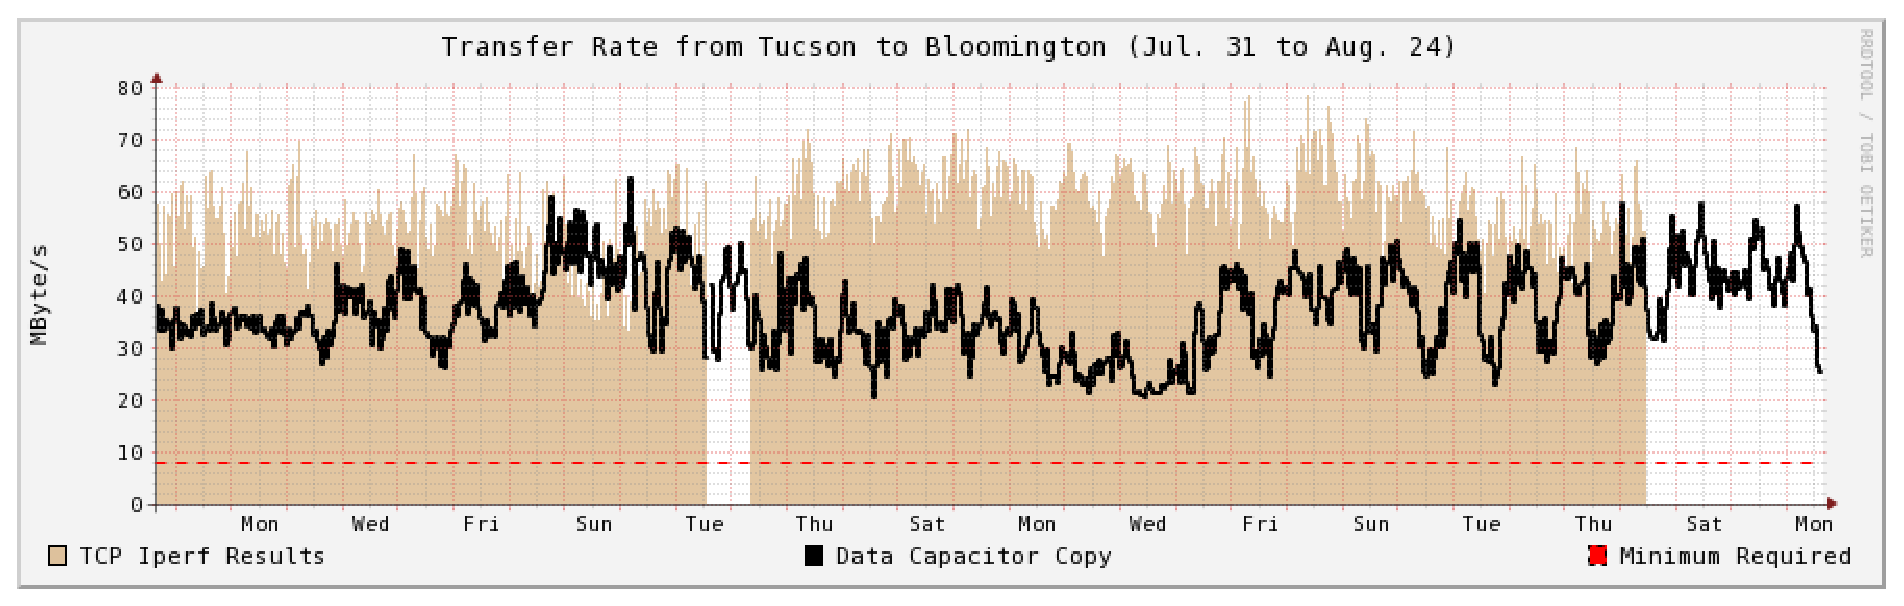
\includegraphics[width=6in]{network_throughput}
\caption{Simulation Results}
\label{fig:network}
\end{figure*}

In our design the network is mainly utilized for three purposes; transferring data from the instrument to the Data Capacitor and archive, transmitting raw data and results during the processing phase, and distributing the data products to individual researchers. Since researches from all over the world can make use of the data products in the archive, it is difficult to characterize the network used to deliver the final data products, we will assume that typical requests for data products will have less bandwidth than we can provide. Due to the fact that the network in this case is highly variable depending on the individual researcher's institution, we will focus on the first two of these purposes. 

The ODI instrument will be installed on the 3.5 meter telescope at the WIYN observatory on Kitt Peak. Once raw data is collected by the instrument it must be transferred to the facility that houses the short to mid-term storage and archive, in this case Indiana University. By using the Lustre filesystem over the WAN we allow the raw data to be transferred by a simple {\tt cp} command. Images can be copied over as they are taken or can be queued to balance the network load. If one assumes a data rate for the compressed raw data of 250 GB per night, then the nominal bandwidth required is 3 MB/s to transfer the data in a 24 hour period. We have performed tests transferring simulated data from the NOAO headquarters facility located in Tucson, Arizona near the Kitt Peak Observatory to the Data Capacitor at IU, and have found that the bandwidth from the NOAO headquarters is more than sufficient to transfer the raw data to the Data Capacitor. Figure \ref{fig:network} shows the results of these tests. The brown bars show the available bandwidth on the network, measured using the TCP iperf network testing software; the black line shows the data rate that can be achieved using standard copy operations with the Lustre file system of the Data Capacitor; the dashed red line represents the required
minimum network bandwidth to be able to transfer an average night�s worth of ODI data to
the Data Capacitor in about 10 hours.

Using the iperf test tool, we determined that the available free bandwidth between Tucson
and Bloomington is between 30 and 80MB/s. With the Lustre file system of the Data Capacitor,
we can achieve a throughput between 20 and 60 MB/s over this connection. We measured
the throughput by copying an actual compressed image with a file size of roughly 1GB from NOAO to
the Data Capacitor. We copied one image every three minutes, for the entire test period throughout the month of August 2009.

For the distribution of raw data sets to the TeraGrid sites that will be used as compute facilities, our plan is to use the TeraGrid network, a dedicated 10G research network. The same network will be used to return the data products resulting from the processing. The Data Capacitor has been used in conjunction with the TeraGrid network to facilitate distributed workflows at several TeraGrid sites including {\bf NEED LIST HERE AND CITATIONS!!!}, and will be used in a similar manner for ODI data. The amount of data to be transferred is of the same order as the amount of raw data, but will include the returned data products and calibration images so may exceed the raw data rate by a factor of two or more. However, this is not anticipated to be a problem with the TeraGrid network since it has an order of magnitude more bandwidth than the NOAO to IU network.

The compute facilities 

The part of the system most visible to the astronomical community will be the science gateway. Science gateways provide a way for entire communities of users to access shared resources through a customized web-accessible interface. Since a science gateway is much more complex than an average website, it does more than simply provide information and links to other websites. Science gateways typically provide access to user data and data collections, community software, workflows, job execution, visualization, and social networking. They are especially useful in increasing productivity by shielding end users from the complexities of accessing data and running jobs on high-end compute resources with varying access mechanism.

Many scientific communities, in all fields, are beginning to use gateways to pool their resources and centralize expertise.  A list of science gateways that use the TeraGrid for compute power can be found at http://teragrid.org/gateways/. Of these, three are for astronomy: the Dark Energy Survey Data Management (DESDM) Gateway, the gateway for the Massive Pulsar Surveys using the Arecibo L-band Feed Array (ALFA), and the Asteroseismic Modeling Portal (AMP).  

The ODI gateway will be very similar in many ways to the LEAD Science Gateway (Linked Environments for Atmospheric Discovery), a TeraGrid Science Gateway developed at IU. LEAD is used by students and researchers for meteorological analysis and modeling. It was developed over 6 years as a research project. By building on this past work, co-opting, customizing, and modifying basic LEAD components, and adding our own specialized modules, we can build a unique and highly productive gateway optimized for ODI.




\subsection{A Detailed Workflow for ODI Images}\label{sec:workflow}

Here we detail the steps in a workflow for processing a set of images. For convenience, we define several conceptual stages of the reduction and analysis called ``Tiers". Each of the Tiers represent different levels of the reduction workflow and require different levels of cyberinfrastructure to support. The Tiers are defined in the ODI Pipeline Software and Archive Science Requirements Document \cite{PASRD} as:
\begin{description}
\item[\bf Tier 0] Real-time (quick look) analysis for observers and (possibly) time-domain
programs: basic analysis done on site on local machines. 
\item[\bf Tier 1] End-of-run, removal of instrument signatures (from master calibrations) and more
advanced spectrometric and photometric calibrations on individual images (1\% flatness).
\item[\bf Tier 2] Production of optimum science products. For example: Image stacking, high
accuracy astrometric and photometric solutions, PSF re-sampling, cosmic ray removal,
fringing correction. Fine-tuning on stacking (e.g. specific selections of images) and
production of catalogs (1\% photometry accuracy).
\item[\bf Tier 3] Image manipulation (for example, image filtering, image arithmetic, marking and
examining sources, artificial star tests), display, photometry, etc.
\end{description}
These Tiers give conceptual distinctions in the overall image processing workflow. Tier 0 is an onsite verification stage which validates the scientific value of the image. Since it is 



At IU, data will reside on both the Data Capacitor (DC) and the Massive Data Storage System (MDSS).
The Data Capacitor will host 200TB of short to mid-term storage for the analysis and production of Tier 1 and Tier 2 data products. Users will be granted quotas based on the projected amount of data that will be collected during their observations. In addition to quotas being granted to users with observing time, some amount of space will be made available to users interested in using archival data only. To prevent overruns on the Data Capacitor space, files that have been pulled from the archive and remain unused for some time will be deleted. However, the user will be able to quickly and easily restore them if they are needed again.

The MDSS will host the ODI archive, which will store all raw science images and calibration data.
Access to data in the archive will be restricted to the PI, and any users that he or she specifies, during the 18 month proprietary period following the observation. After this time, the raw data will become public. The PMD will contain searchable metadata entries for the data products, as well as the metadata for the processing itself (the workflow). The latter will allow the reproduction of data products from the raw archived data. 

Data transfer from the WIYN telescope to IU begins once an observation has been taken, the data and metadata files are available, and the transfer to the Data Capacitor has been queued. 
The summit facility will have a small disk buffer that will provide two weeks of raw data storage to smooth the data flow and mitigate interruptions due to network outages and system maintenance. As detailed in \S\ref{sec:components} we have established a stable Data Capacitor mount from Tucson to IU which can meet the required data transfer rate. Next, the metadata file is ingested into the PMD. This is followed by copying the files from the Data Capacitor to the archive. Once this transfer is completed, the PMD communicates to the summit local buffer that the files have been replicated. They are then deleted from the local buffer and the transfer is removed from the queue.

New images are queued for Tier 1 processing by OGCE following the ingestion of the metadata and the verification of the files on the DC and MDSS. 
Based on the metadata associated with the image (e.g., observing mode, filter, moon phase, etc.), appropriate master calibrations and processing parameters are selected. The proper parameters for the processing engine and the TeraGrid resource best suited for the job are determined based on these selections. The workflow system then takes the input data, calibration data, and run parameters and generates the appropriate batch submission script for the TeraGrid resource that will run the job. For TeraGrid resources with Data Capacitor access the input data will already be available on the supercomputer. The job is executed on the TeraGrid resource and the results are written back to the Data Capacitor. The metadata is then updated with information about the job, as well as statistics of the result data. Once the Tier 1 processing has been confirmed the PI is notified. The PI can then log into the science gateway to view his or her Tier 1 processed data and begin Tier 2 processing or initiate a download.

Tier 1 data products will exist temporarily on the Data Capacitor, as it is a users' workspace. If the data are not accessed by the PI for some period of time, they will be migrated off of the DC. The processing metadata for the confirmed Tier 1 run will be saved so that the Tier 1 data products can be re-created using the same workflow, i.e., the same processing steps, parameters, and calibration data. This re-creation will occur seamlessly as needed, without the need for user interaction. The only indication of the reprocessing would be a delay in the initiation of a Tier 2 workflow or Tier 1 download.



One important and basic function of the ODI Gateway will be to enable users to browse and search their data.  When users log in to the gateway, they will be able to to see and select among their files by clicking in an expandable directory tree. Actually, the ''files'' will be complete images composed of multiple .fits files, and the directory structure on the DC will not necessarily be the same as that displayed, but the gateway will deal with all these details, making things clearer and more convenient for users. When one clicks on a file in the tree, the metadata about that image (or table or other item) will be displayed. Thumbnails and larger versions of images will be available for display, as well.  
Searching for data will involve searching the metadata in the PMD to find observations, calibrations, or tables that have desired characteristics. One might, for example, search for all observations of M31 taken with a certain filter using a specific observing mode.  The same methods will be used to search the archive data as are used to search private files. 

The ODI Science Gateway will also provide Tier 2 processing that is initiated and controlled by astronomers. To begin, the user will select one or more Tier 1 (or previously-made Tier 2) images as input, then invoke the graphical workflow builder, probably the most novel aspect of the gateway from the point of view of most astronomers. 
Workflows consist of an operation or set of operations to be carried out on input data. Pre-made ODI workflows that will be provided include stacking, differencing, slicing, object identification, photometry, and astrometry. Each will have a set of default parameters determined by the pipeline scientist to produce the best results for the broadest range of astronomical applications, but the user will be able to modify the settings if the need arises. Using drag-and-drop, a user will be able to select one or more pre-made workflows and arrange them in a desired order, connecting the input files to the the first task and wiring the others together, outputs to inputs (e.g., stack several narrow-band images and several broad-band images, then do a difference of the stacks). The arrangements may become quite complex. Forms in which to enter or edit required parameter settings will be constructed automatically. One will be able to save these user-made workflows for reuse and sharing.  Users will also be able to access the individual OIPP modules that make up the pre-made workflows, to compose more intricate workflows. In this way, users may exclude parts of a pre-made workflow that adversely influence their results.

Once a user has finalized his or her workflow and set all of the processing parameters, the workflow engine will dispatch the job to an appropriate TeraGrid resource. Although ODI image processing will occur on TeraGrid supercomputers, gateway users will not have TeraGrid accounts and will need know nothing about the complex process of running jobs on the TeraGrid. The gateway will submit jobs using a community account, take care of all the authorization and file movement details, and track resource usage by individuals. The workflow builder will also be able to monitor the progress of a running job. In ''monitoring mode,'' it will display notifications from the applications running on the TeraGrid. The status of all of a user's submitted jobs will also be displayed in the science gateway at login, and the user may elect to be notified by email when a job completes. 
 
Results from Tier 2 workflows will be stored in the user workspace on the DC, available for download or for use as inputs to subsequent workflows. Before downloading, it will be possible to downsample or cut out sections of an image to limit the volume of data that has to be transferred then stored locally. Like Tier 1 data products, Tier 2 results will be moved off of the Data Capacitor after a number of weeks to allow the widest possible use of the system and to meet storage quotas. However, data products that are being accessed will not be deleted. Those that are deleted will still appear in the user's view in the science gateway but will be flagged as not being immediately available. Using the metadata saved for each workflow, data products will be reproduced as needed.   

Although the proposed solution is similar in some ways to existing pipeline and archive facilities, our design incorporates several advances which make it a state-of-the-art solution. Early in the design process it was recognized that ODI data sets will be extremely large, complex, and difficult to work with, perhaps overwhelmingly so for individual users. Not only are the data volumes immense, but the complexity of dealing with 4096 {\tt .fits} extensions is significantly greater than what is experienced with typical mosaic imagers. It was also realized that simply delivering Tier 1 data products, via download or media, would not alleviate most of these difficulties. Due to these facts, we determined that the proposed solution should enable the end user to get as close as possible to the final scientific results of their workflow before requiring them to be responsible for receiving, storing and manipulating the data on their own. 

In this way the proposed solution differs substantially from most currently existing pipeline and archive facilities. Typically such facilities provide a data product, available for download or delivery, which a scientist can then manipulate to achieve his science goals. These facilities provide data products, {\bf not} a data reduction service, which is what the proposed solution endeavors to do. In this respect, the proposed solution will go far beyond current offerings. We will provide the data products, network connectivity, hardware, archival storage, and the necessary software toolkit to achieve many science goals. For many science programs the proposed system will truly be an end-to-end system.

Our design will also incorporate and enable additional features such as the inclusion of user contributed modules and community tools to enable and encourage collaboration on ODI projects. We will detail a process whereby users can develop their own modules that adhere to the OIPP programming guidelines. After review by the pipeline scientists and programmers, these modules will be included and maintained by the OIPP pipeline staff. Community tools such as live messaging, forums, standardized workflows, etc. will be available via the science gateway. Users may, of course, decide to remain anonymous and opt out of these community tools if they wish. 

\section{Future Directions}\label{sec:future}

\section{Conclusion}\label{sec:conclusion}


% An example of a floating figure using the graphicx package.
% Note that \label must occur AFTER (or within) \caption.
% For figures, \caption should occur after the \includegraphics.
% Note that IEEEtran v1.7 and later has special internal code that
% is designed to preserve the operation of \label within \caption
% even when the captionsoff option is in effect. However, because
% of issues like this, it may be the safest practice to put all your
% \label just after \caption rather than within \caption{}.
%
% Reminder: the "draftcls" or "draftclsnofoot", not "draft", class
% option should be used if it is desired that the figures are to be
% displayed while in draft mode.

% Note that IEEE typically puts floats only at the top, even when this
% results in a large percentage of a column being occupied by floats.


% An example of a double column floating figure using two subfigures.
% (The subfig.sty package must be loaded for this to work.)
% The subfigure \label commands are set within each subfloat command, the
% \label for the overall figure must come after \caption.
% \hfil must be used as a separator to get equal spacing.
% The subfigure.sty package works much the same way, except \subfigure is
% used instead of \subfloat.
%
%\begin{figure*}[!t]
%\centerline{\subfloat[Case I]\includegraphics[width=2.5in]{subfigcase1}%
%\label{fig_first_case}}
%\hfil
%\subfloat[Case II]{\includegraphics[width=2.5in]{subfigcase2}%
%\label{fig_second_case}}}
%\caption{Simulation results}
%\label{fig_sim}
%\end{figure*}
%
% Note that often IEEE papers with subfigures do not employ subfigure
% captions (using the optional argument to \subfloat), but instead will
% reference/describe all of them (a), (b), etc., within the main caption.


% An example of a floating table. Note that, for IEEE style tables, the 
% \caption command should come BEFORE the table. Table text will default to
% \footnotesize as IEEE normally uses this smaller font for tables.
% The \label must come after \caption as always.
%
%\begin{table}[!t]
%% increase table row spacing, adjust to taste
%\renewcommand{\arraystretch}{1.3}
% if using array.sty, it might be a good idea to tweak the value of
% \extrarowheight as needed to properly center the text within the cells
%\caption{An Example of a Table}
%\label{table_example}
%\centering
%% Some packages, such as MDW tools, offer better commands for making tables
%% than the plain LaTeX2e tabular which is used here.
%\begin{tabular}{|c||c|}
%\hline
%One & Two\\
%\hline
%Three & Four\\
%\hline
%\end{tabular}
%\end{table}


% Note that IEEE does not put floats in the very first column - or typically
% anywhere on the first page for that matter. Also, in-text middle ("here")
% positioning is not used. Most IEEE journals/conferences use top floats
% exclusively. Note that, LaTeX2e, unlike IEEE journals/conferences, places
% footnotes above bottom floats. This can be corrected via the \fnbelowfloat
% command of the stfloats package.




% conference papers do not normally have an appendix


% use section* for acknowledgement
\section*{Acknowledgment}


The authors would like to thank... \cite{simms2007}





% trigger a \newpage just before the given reference
% number - used to balance the columns on the last page
% adjust value as needed - may need to be readjusted if
% the document is modified later
%\IEEEtriggeratref{8}
% The "triggered" command can be changed if desired:
%\IEEEtriggercmd{\enlargethispage{-5in}}

% references section

% can use a bibliography generated by BibTeX as a .bbl file
% BibTeX documentation can be easily obtained at:
% http://www.ctan.org/tex-archive/biblio/bibtex/contrib/doc/
% The IEEEtran BibTeX style support page is at:
% http://www.michaelshell.org/tex/ieeetran/bibtex/
%\bibliographystyle{IEEEtran}
% argument is your BibTeX string definitions and bibliography database(s)
%\bibliography{IEEEabrv,../bib/paper}
%
% <OR> manually copy in the resultant .bbl file
% set second argument of \begin to the number of references
% (used to reserve space for the reference number labels box)
\bibliographystyle{IEEEtran}
\bibliography{general}


% that's all folks
\end{document}


